1. Explain finite difference methods.
2. Derive the numerical methods and their truncation error (show error behaviour).

Methods included:
1. One-step method
    a. Euler's explicit
    b. Euler's implicit
    c. 4-stage Runge-Kutta method
    d. trapezium rule
    remarks: fixed point iteration method included to compute implicit methods
2. Predictor-corrector method
    a. Euler-trapezium method
3. Adaptive method
    a. ode23 method (Matlab)
    b. ode45 method (Matlab)
    
%---------------------------------------------------------------------------------
\chapter{Numerical methods}
\label{chap:numerical-methods}
%---------------------------------------------------------------------------------
In real world problems, ODE systems are frequently used. However, these models cannot be solved analytically. Therefore, the solution has to be estimated by numerical methods. The most popular and simple method is the Euler's method.

Intuitively, the Euler's explicit method tries to estimate the value at the next step following the gradient of the solution at current point. If the step size is sufficiently small, the estimation will be accurate.

An initial value problem, has the general form of 
\begin{align}
    y'&=f(x,y)\\
    y(x_0) &= y_0
\end{align}
for $x \in [x_0, X_M]$.

Notation:
Throughout the report, we will use the following notation.
$y_n$ - numerical approximation of $y(x_n)$
$y(x_n)$ - analytical solution at mesh point $x_n$
$x_n$ - mesh points of defined range, where

\begin{align}
    x_n &= x_0 + nh\\
    h &= \frac{(X_M - x_0)}{N}
\end{align}

for $n = 0,\dots, N$

\section{One-step methods}
For the simple Euler's explicit method, 
\begin{equation}
    y_{n+1} = y_n + hf(x_n,y_n)\\
\end{equation}

The implementation is as follows:

\begin{lstlisting}[language=Python]
y_n = [self.initial_value]
x_n = [self.x_min]

# Calculate approximated solution for each mesh point.
for n in range(1, self.mesh_points + 1):
    step = [self.mesh_size * f for f in self.func(x_n[-1], y_n[-1])]
    y_n.append([a + b for a, b in zip(y_n[-1], step)])
    x_n.append(self.x_min + n * self.mesh_size)

return x_n, y_n
\end{lstlisting}

The truncation error is defined to be the difference of exact solution with the numerical solution given the exact solution of previous mesh point is known. Therefore, we have that the truncation error for Euler's explicit method to be

\begin{equation}
\label{eqn:trun_err_def}
    T_n \defeq \frac{y(x_{n+1}) - y(x_{n})}{h} - f(x_n, y(x_n))
\end{equation}

According to Taylor's series expansion, we have 
\begin{equation}
    y(x_n + h) = y(x_n) + hy'(x_n) + \frac{1}{2}h^2y''(\xi_n)
\end{equation}
for $\xi_n \in (x_n, x_{n+1})$. Substitute this to the truncation error, noting that $f(x_n, y(x_n)) = y'(x_n)$ we get
\begin{equation}
    T_n = \frac{1}{2}h^2y''(\xi_n)
\end{equation}

Therefore, the truncation error for Euler's explicit method varies linearly with the step size.

In this report, we will use an example model 
\begin{align}
\label{eqn:example_model}
    f(x,y) &= -y \\
    y(x_0) &= 1
\end{align}
for $x \in [0, 5]$ to show that the implementation follows the theory.

Some examples of the solution to the given model can be found here: \href{https://nbviewer.jupyter.org/github/FarmHJ/numerical-solver/blob/main/examples/solver_convergence.ipynb}{Example model notebook}

Result image extracted from the notebook above shows that the truncation error follows 

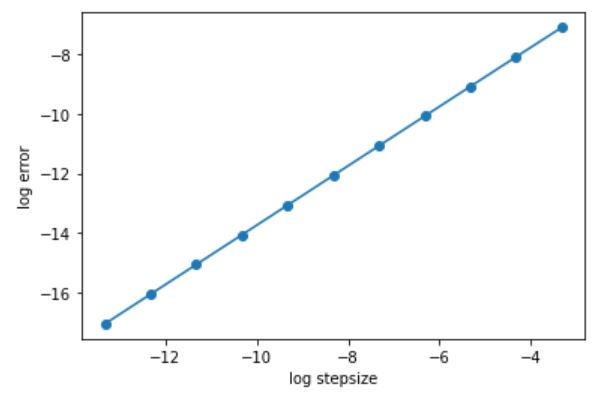
\includegraphics[width=0.95\columnwidth]{Euler_explicit_error_behaviour}

Other than the Euler's explicit method, the other one-step methods implemented are the Euler's implicit method, trapezium rule method and four-stage explicit Runge-Kutta method.

The Euler's implicit method is defined to be
\begin{equation}
    y_{n+1} = y_n + hf(x_{n+1},y_{n+1})\\
\end{equation}
, while the trapezium rule method is
\begin{equation}
    y_{n+1} = y_n + \frac{1}{2}h[f(x_n,y_n) + f(x_{n+1},y_{n+1})]\\
\end{equation}
. These methods, including Euler's explicit method, Euler's implicit method and trapezium rule method, can be generalised under the $\theta$-method,
\begin{equation}
    y_{n+1} = y_n + h[(1-\theta)f(x_n,y_n) + \theta f(x_{n+1},y_{n+1})]\\
\end{equation}
. For $\theta = 0$ and $\theta = 1$, the methods are Euler's explicit and Euler's implicit method respectively. Using the same definition for truncation error in \ref{eqn:trun_err_def}, we can see that the truncation error are $T_n = -\frac{1}{2}hy''(\xi_n)$ for $\xi_n \in (x_n, x_{n+1})$ and $T_n = -\frac{1}{12}h^2y^{(3)}(\xi_n)$ for $\xi_n \in (x_n, x_{n+1})$ respectively.

The Euler's implicit method implementation,
\begin{lstlisting}[language=Python]
y_n = [self.initial_value]
x_n = [self.x_min]

# Use value at previous mesh point as prediction for
# fixed point iteration if no prediction is given.
if prediction is None:
    prediction = y_n[-1]

# Calculate approximated solution for each mesh point.
# Use fixed point iteration to solve numerical equation.
for n in range(1, self.mesh_points + 1):

    def num_method(prediction):
        step = [self.mesh_size * f for f in self.func(
            x_n[-1] + self.mesh_size, prediction)]
        return [a + b for a, b in zip(y_n[-1], step)]

    est_y = self.fixed_pt_iteration(prediction, num_method)
    y_n.append(est_y)
    x_n.append(self.x_min + n * self.mesh_size)

return x_n, y_n
\end{lstlisting}

The trapezium rule method implementation,
\begin{lstlisting}[language=Python]
y_n = [self.initial_value]
x_n = [self.x_min]

# Use value at previous mesh point as prediction for
# fixed point iteration if no prediction is given.
if prediction is None:
    prediction = y_n[-1]

# Calculate approximated solution for each mesh point.
# Use fixed point iteration to solve numerical equation.
for n in range(1, self.mesh_points + 1):

    def num_method(prediction):
        previous_func = self.func(x_n[-1], y_n[-1])
        new_func = self.func(x_n[-1] + self.mesh_size, prediction)
        return [a + self.mesh_size / 2 * (b + c) for a, b, c in zip(
            y_n[-1], previous_func, new_func)]

    est_y = self.fixed_pt_iteration(prediction, num_method)
    y_n.append(est_y)
    x_n.append(self.x_min + n * self.mesh_size)

return x_n, y_n
\end{lstlisting}

When these methods are tested on the example model \ref{eqn:example_model}, the truncation error does not behave as expected. This is probably due to the use of fixed point iteration algorithm to estimate the solution of implicit functions. The error graph is shown below.

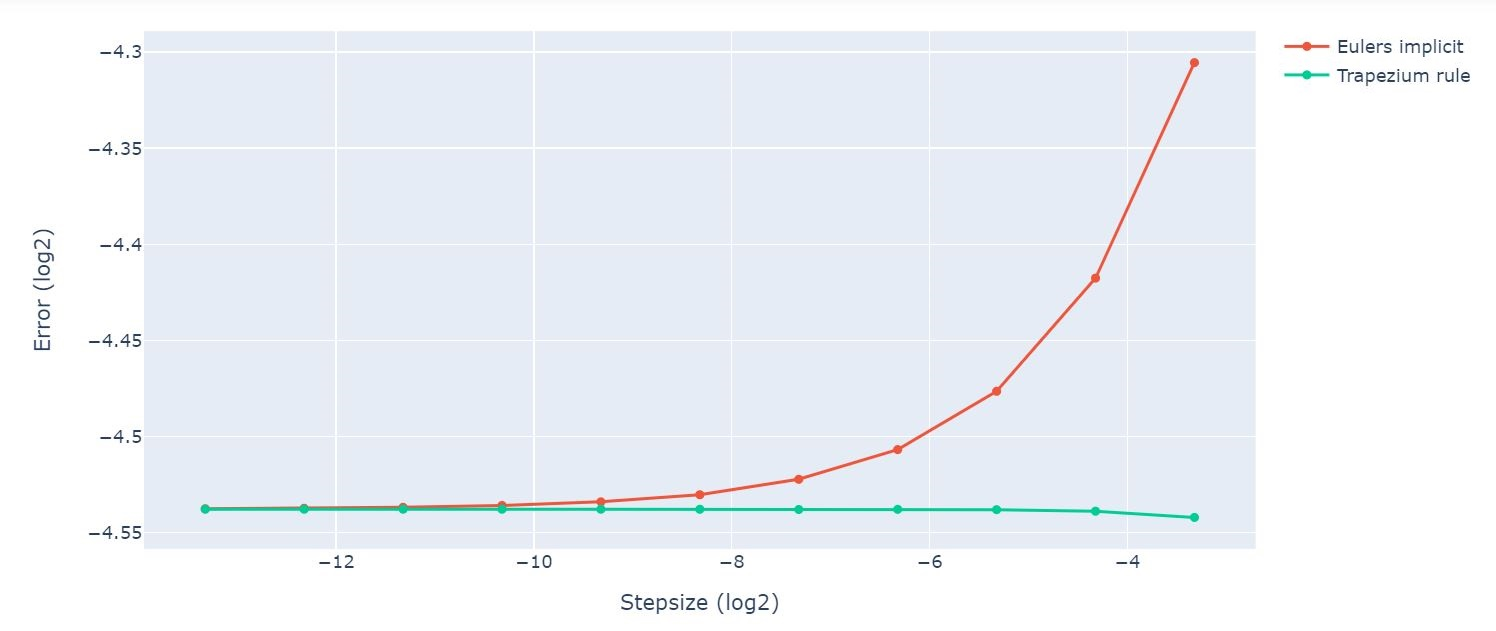
\includegraphics[width=0.95\columnwidth]{Eulerimplicit_trapezium_error_behaviour}

\section{Predictor-corrector methods}
For the implicit methods, numerical value at previous mesh point is chosen as the initial value for the fixed point iteration algorithm. The predictor-corrector method suggests a more carefully chosen initial guess for the implicit methods. An explicit numerical method is used as a predictor of the initial value of an implicit method. The initial value is then used as an initial guess for iterations to solve an implicit function. The implicit method that refines the solution is known as the corrector method. The Euler-Trapezoidal method is a predictor-corrector that uses an Euler's explicit method as the predictor and trapezium rule method as the corrector. In this implementation, the trapezium rule method corrector is iterated until a set of conditions are satisfied. The conditions are defined to be the difference between current iteration and previous iteration is lesser than a given threshold value or the number of iterations exceeds a certain amount.  